\subsection{Caso d'uso UC6: Esportazione del progetto}
	\begin{figure}[h]
		\centering
		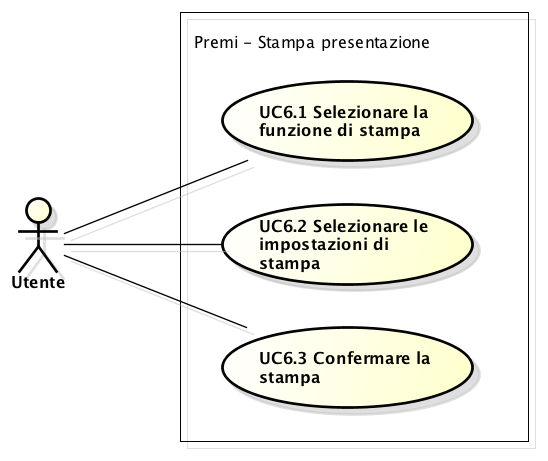
\includegraphics[scale=0.45] {img/UC6.png}
		\caption{UC6 - Esportazione del progetto}
	\end{figure}

	\begin{itemize}
		\item \textbf{Attori:} Utente autenticato;
		\item \textbf{Scopo e descrizione:} L'utente ha aperto un progetto e vuole esportarlo in locale per poterlo visualizzare offline;
		\item \textbf{Precondizione:} Il sistema è in attesa che l'utente selezioni la funzione esporta;
		\item \textbf{Flusso principale degli eventi:}
		\begin{enumerate}
			\item L'utente seleziona dal menù la funzione esporta [UC6.1];
			\item Il sistema prepara il pacchetto da esportare [UC6.2]
			\item L'utente salva il pacchetto in locale [UC6.4];
		\end{enumerate}
		\item \textbf{Postcondizione:} L'utente ha esportato il progetto e l'ha salvato in locale.
	\end{itemize}


\subsection{Caso d'uso UC6.1: Selezionare la funzione esporta}
	\begin{itemize}
		\item \textbf{Attori:} Utente autenticato;
		\item \textbf{Scopo e descrizione:} L'utente seleziona dall'apposito menù la funzione di esportazione per esportare il progetto;
		\item \textbf{Precondizione:} L'utete ha un progetto aperto e il sistema è in attesa che l'utente selezioni la funzione esporta;
		\item \textbf{Postcondizione:} Il sistema inizia la procedura di esportazione.
	\end{itemize}


\subsection{Caso d'uso UC6.2: Preparazione del pacchetto da esportare}
	\begin{itemize}
		\item \textbf{Attori:} Sistema;
		\item \textbf{Scopo e descrizione:} Il sistema prepara il pacchetto da salvare in locale contenente il progetto;
		\item \textbf{Precondizione:} L'utente ha scelto di esportare il progetto;
		\item \textbf{Postcondizione:} Il sistema ha preparato il pacchetto del progetto e lo ha salvato nel server.
	\end{itemize}


\subsection{Caso d'uso UC6.3: Salvataggio del pacchetto in locale}
	\begin{itemize}
		\item \textbf{Attori:} Utente autenticato;
		\item \textbf{Scopo e descrizione:} L'utente deve salvare il pacchetto del progetto memorizzato sul server in locale.
		\item \textbf{Precondizione:} Il sistema ha preparato il pacchetto, il quale si trova sul server;
		\item \textbf{Postcondizione:} Il pacchetto è stato scaricato e salvato in locale.
	\end{itemize}